\documentclass{school-22.101-notes}
\date{October 19, 2011}

\begin{document}
\maketitle


\topic{Analytical Relations between $V_0, r_0, E_B$ \label{2H-relation}}
In this section we consider an easiest form of nucleon-nucleon potential (the interaction between a neutron and a proton): a spherical well as in Fig.~\ref{deuteron-potential}, assume s-wave ($l=0$),
\eqn{ V(r) = \left\{ \begin{array}{cc} -V_0 & r \le r_0 \\ 0 & r > r_0   \end{array} \right. }
\begin{figure}[h!]
    \centering
    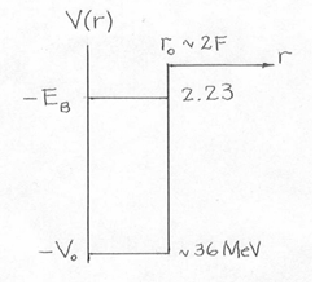
\includegraphics[width=2in]{images/deuteron/deuteron-potential.png}
    \caption{Deuteron Potential Well} \label{deuteron-potential}
\end{figure}

We solve for analytical relations between the well depth $V_0$, well width $r_0$, and binding energy $E_B$: 
\begin{enumerate}
\item From the eigenvalue problem, $l=0$ gets rid of the $L^2$ term:
\eqn{   \left[ - \frac{\hbar^2}{2 \mu}  \pprn2  +  V_{\mathrm{nuc}} (r) - E_n  \right] u_n (r)  = 0  }
in which $E<0$ (bound state), and the potential well of $-V_0$ goes from $0$ to $r$, and $-V_0 < E < 0$. 

\item Write out general form of solutions:  
\begin{enumerate}
\item For $r \le r_0$, notice $E - (-V_0) = E + V_0$. 
\eqn{ u_n (r) &= A \sin k_1 r + B \cos k_1 r  & k_1 &= \frac{\sqrt{2 \mu (E+V_0)}}{\hbar} }

\item For $r > r_0$, 
\eqn{ u_n (r) = C e^{-k_2 r} + D e^{k_2 r} }
\end{enumerate}

\item Apply boundary conditions:
\begin{enumerate}
\item Recall $\psi_n (r) = \frac{u_n(r)}{r}$, then 
\eqn{ \psi_n (r=0) \neq \infty \Rightarrow  u_{nl} (r=0) = 0 \Rightarrow B = 0}

\item Using symmetry:
\eqn{ \psi_n (r \to \infty) \neq \infty \Rightarrow u_{nl} (r\to \infty) = 0 \Rightarrow D = 0}
If we were to distinguish between the two sides of the well, then to the right of the well $u_n(x) = C e^{-k_2 x}$, and to the left of the well $u_n (x) = C' e^{k_2 x}$. 
\end{enumerate}

\item Apply interface conditions: $\psi_n, \psi^{\prime}_n$ are continuous at $r_0$: 
\eqn{ \Rightarrow k_1 \cot (k_1 r_0) = - k_2 }
Notice this is the same as the odd-parity square well problem in Chapter~\ref{finite-square-well}. 


\item We reach a transcendental equation describing the dependency of $V_0, r_0, E_B$ on each other:
\eqn{ \boxed{ \cot (k_1 r_0 ) = -\frac{k_2}{k_1} = - \sqrt{\frac{-E}{E+V_0}}  } \label{H2-V_0}}

\item Estimation of $V_0$. 
  \begin{enumerate}
  \item The minimum depth of a well, that is, a barely bound state:
    \begin{enumerate}
    \item A barely bound state means $\displaystyle E \to 0, |V_0| \gg |E|, \cot (k_1 r_0) \to 0, k_1 r_0 \simeq \frac{\pi}{2}$. 
    \item Alternatively, we can also consider, for outside the well to decrease, the width of the well has to be at least 1/4 of the $\sin$ wave: $\displaystyle r_0 \gtrsim \frac{1}{4}\lambda = \frac{1}{4}\frac{2 \pi}{k_1}  = \frac{\pi}{2k_1}  \Rightarrow k_1 \gtrsim \frac{\pi}{2} \frac{1}{r_0} $
    \end{enumerate}
    Together, that is to say,
    \eqn{ \mathrm{KE} = \frac{\hbar^2 k_1^2}{2\mu} = \frac{\hbar^2 \pi^2}{8 \mu r_0^2} < V_0 \Rightarrow V_0 > \frac{\hbar^2 c^2}{\mu c^2} \frac{\pi^2}{8 r_0^2} = \frac{ (197 \fsp \MeV \fm )^2}{469 \MeV} \frac{\pi^2}{8 \times (2.1 \fsp \fm)^2 } = 23 \fsp \MeV  }

  \item The actual well depth of a Deuteron: using measured $r_0, E_B$, we can find $V_0$ using Eq.~\ref{H2-V_0}:
    \begin{enumerate}
    \item $r_0$ can be measured from the scattering experiment. For \ce{^2H}, $r_0 = 2.1 \fm$. 
    \item The binding energy $E = -2.22$ MeV. We can measure $E_B$ through: 
      \begin{itemize}
      \item mass spectroscopy;
      \item measure the $\gamma$ energy in p + n $\to$ \ce{^2 H} + $\gamma$;
      \item measure the $\gamma$ energy in $\gamma +$ \ce{^2H} $\to$ n + p;
      \end{itemize}
      The $2.22 \fsp \MeV$ binding energy is for ground state \ce{^2H} (we can tell it is ground state because excited states decay very rapidly). A binding energy of $2.22 \fsp \MeV$ is rather weak, because the average nucleus binding energy is $8 \fsp \MeV$. 

    \item We can solve for $k_1 r \simeq 1.8305$, then the well depth of a deuteron is $V_0 = 35 \fsp \MeV$.
    \end{enumerate}
  \end{enumerate}


\item The sign of $E$ is the ultimate measurement of whether a state is bounded or not. 
\begin{enumerate}
\item Ground state has a total energy of $E = -2.22 $ MeV, which is smaller than the averaged -8 MeV, hence the ground state of deuteron weakly bounded. 
\item The 1st excited state has a total energy of $E = 265$ MeV, hence is it not bounded. Thus it is virtual. 
\end{enumerate}
See Figure~\ref{deuteron-bound} for details. 

\begin{figure}
    \centering
    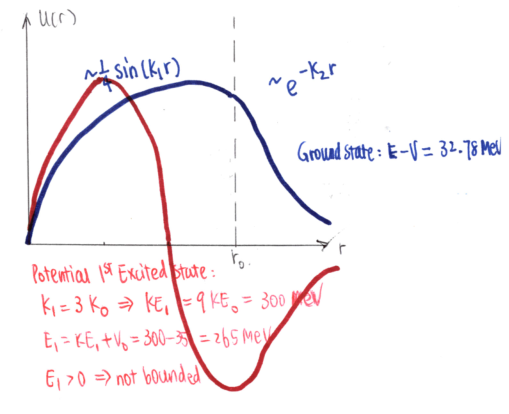
\includegraphics[width=5in]{images/deuteron/deuteron-states.png}
    \caption{Deutrium Ground State, 1st Excited State Potential Energy}    \label{deuteron-bound}
\end{figure}

\item Higher angular momentum states cannot be bounded (mostly):
\eqn{ V_{\mathrm{angular \fsp momentum \fsp barrier}} = \frac{\hbar^2 l (l+1)}{2 \mu r^2} }
\eqn{ \Delta V^{\mathrm{min}}_{l=1} =  \frac{\hbar^2 l (l+1)}{2 \mu r^2} =  \frac{\hbar^2 c^2}{\mu c^2 r^2} = \frac{(197 \fsp \MeV \fm)^2}{(469 \fsp \MeV) (2.1\fsp \fm)^2} = 18.8 \fsp \MeV > 2.2 \fsp \MeV }
The additional potential needed for $l=1$ is 18.8 MeV, larger than the 2.2 MeV available, thus \textbf{$l \ge 1$ cannot be bound state for \ce{^2H}}. 
\end{enumerate}



%%%%%%%%%%%%% Spin Dependence %%%%%%%%%%%%%%%%%%%%%%%
\topic{Spin of Deuteron, S-S Coupling, Spin Dependence of Nuclear Force \label{2H-spin}}
The spin dependence of nuclear forces can be interpreted as $V_{\mathrm{nuc}}$ depends on whether spin is parallel or anti-parallel. More specifically, 
\begin{itemize}
    \item In the context of (n,p) deuteron, bound and virtual states (s-s coupling);
    \item In the context of n-p scattering, where spin dependence of $V_{\mathrm{nuc}}$ accounts for the measured scattering cross section (s-l coupling). 
\end{itemize}


 We will discuss more on the spin dependence in Section~\ref{spin-scattering}. 
From measurements, deuteron ground state is mostly $J=1$, also possibly $J=0$.  $S_p = S_n = \frac{1}{2}, \Jhat = \Lhat \oplus \Shat_p \oplus \Shat_n$.
\begin{enumerate}
\item For $J=1$, $l=0$, the possible angular momentum combinations that give us $J=1$ are: $S=1, L=0; S=0, L=1; S=1, L=1; S=1, L=2$. From observation/measurements, we know ground state of deuteron has even parity: recall from the perturbation operator, we derived that the angular momentum parity $\Pi = 1^+$,  and recall parity's definition $\Pi = (-1)^l$; that is, only the ones with even $L$ can exist (so only option 1 and 4 is possible).

\item For $J=0$, we can have $l=0, s=0$. 

\item We consider the $l=0$ case (this is 96\% of the time), then the possible spin configurations are(using notations $\ket{s m}$)\footnote{Griffiths p.185, Liboff Table 11.3}: 
\begin{align}
\left. \begin{array}{l} 
\ket{1 1} = \up \up \\
\ket{1 0} = \frac{1}{\sqrt{2}} (\up \down + \down \up ) \\
\ket{1 -1} = \down \down
\end{array} \right\}
S &= 1  (\mathrm{triplet, parallel, bounded}). \\
\left. \ket{0 0} = \frac{1}{\sqrt{2}} (\up \down - \down \up ) \right\} 
S &= 0  (\mathrm{singlet, antiparallel, unbounded}).
\end{align}

Then we can add a spin-dependent modification to $V_{\mathrm{nuc}}$:
\eqn{ V_{\mathrm{nuc}} (r) = V_0 (r) + V_1 (r) \frac{\Shat_p \cdot \Shat_n}{\hbar^2}  }

We can compute the modification for $(n,p)$ interaction:
\begin{align*}
\Shat &= \Shat_p + \Shat_n \\
\Shat^2 &= (\Shat_p + \Shat_n )(\Shat_p + \Shat_n) = \Shat_p^2 + \Shat_n^2 + 2 \Shat_p \cdot \Shat_n \\
\Shat_p \cdot \Shat_n &= \frac{1}{2} (\Shat^2 - \Shat_p^2 - \Shat_n^2) \\
\expect{\Shat_p \cdot \Shat_n}&= \frac{1}{2} (S(S+1) - S_p (S_p+1) - S_n (S_n+1) ) 
= \left\{ \begin{array}{ccc} S=0 & -\frac{3}{4} \hbar^2 & \mbox{Singlet} \\ S=1 & \frac{1}{4} \hbar^2 & \mbox{Triplet} \end{array} \right. \\
\Aboxed{V_{\mathrm{nuc}} &=  \left\{ \begin{array}{ccccc} 
V_0 (r) - \frac{3}{4} V_1(r)  & \mbox{Singlet}& \mbox{Weaker interaction, virtual} & E^* = 0.077 \fsp \MeV & V_S = -23 \fsp \MeV \\ 
V_0 (r) + \frac{1}{4} V_1(r)  & \mbox{Triplet}& \mbox{Stronger interaction, bound} & E_B = -2.2 \fsp \MeV & V_T = -35 \fsp \MeV
\end{array}\right. } \\
\end{align*}
\begin{figure}[ht]
    \centering
    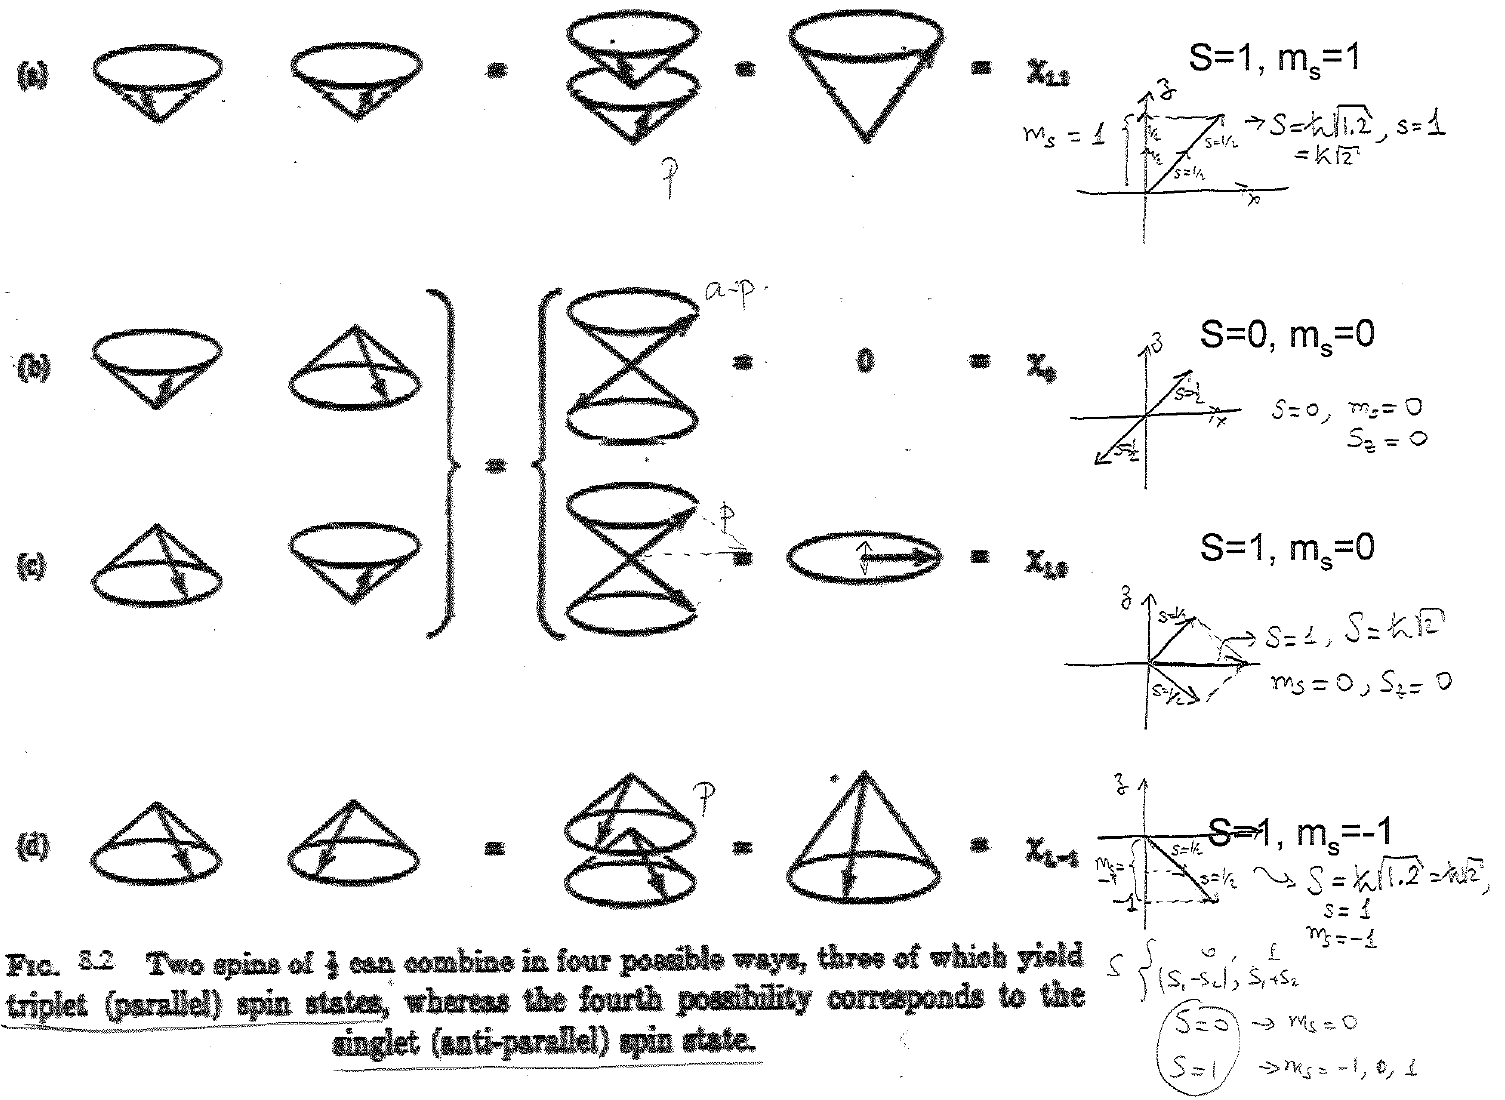
\includegraphics[width=5in]{images/deuteron/deuteron-possible-config.png}
    \caption{Possible Configurations for Two Spin 1/2 Particles}
\end{figure}

Comments:
\begin{enumerate}
\item How spin dependency affects the scattering cross sections: $\sigma_{S=0} = 67.8 \barn, \sigma_{S=1} = 4.6 \barn \Rightarrow \sigma = \frac{3}{4} \sigma_{S=1} + \frac{1}{4} \sigma_{S=0} = 20.4 \barn$. 

\item $E^*, E_B$ are measured results. Then we can calculate the well depths $V_S, V_T$ using $E, r$ (recall last section). 

\item Then we can solve for $V_0, V_1$ from $V_S, V_T$: $V_0 = -32 \fsp \MeV, V_1 = -12 \fsp \MeV$. $V_0 <0, V_1 <0$ meaning they are both positive/attractive. $|V_0| > |V_1|$ means spin dependence is weaker than the spin-independent part. But both are significant contribution. 

\item Only the triplet states are bounded for two reasons: one is that a singlet bound state of deuteron is not observed; the other is the different measurement values of $\sigma_s^s, \sigma_s^p$ (next lecture);

%\item If n-p force is spin-independent, we would expect to find deuteron bound state with $s=1$ at the same energy; but find no $s=0$ bound state. 
\end{enumerate} 
\end{enumerate}








\end{document}
